
\begin{figure*}[ht]
 \centering
    \subfloat[Guided Proofreading Results\label{fig:cylinder_results}]{%
      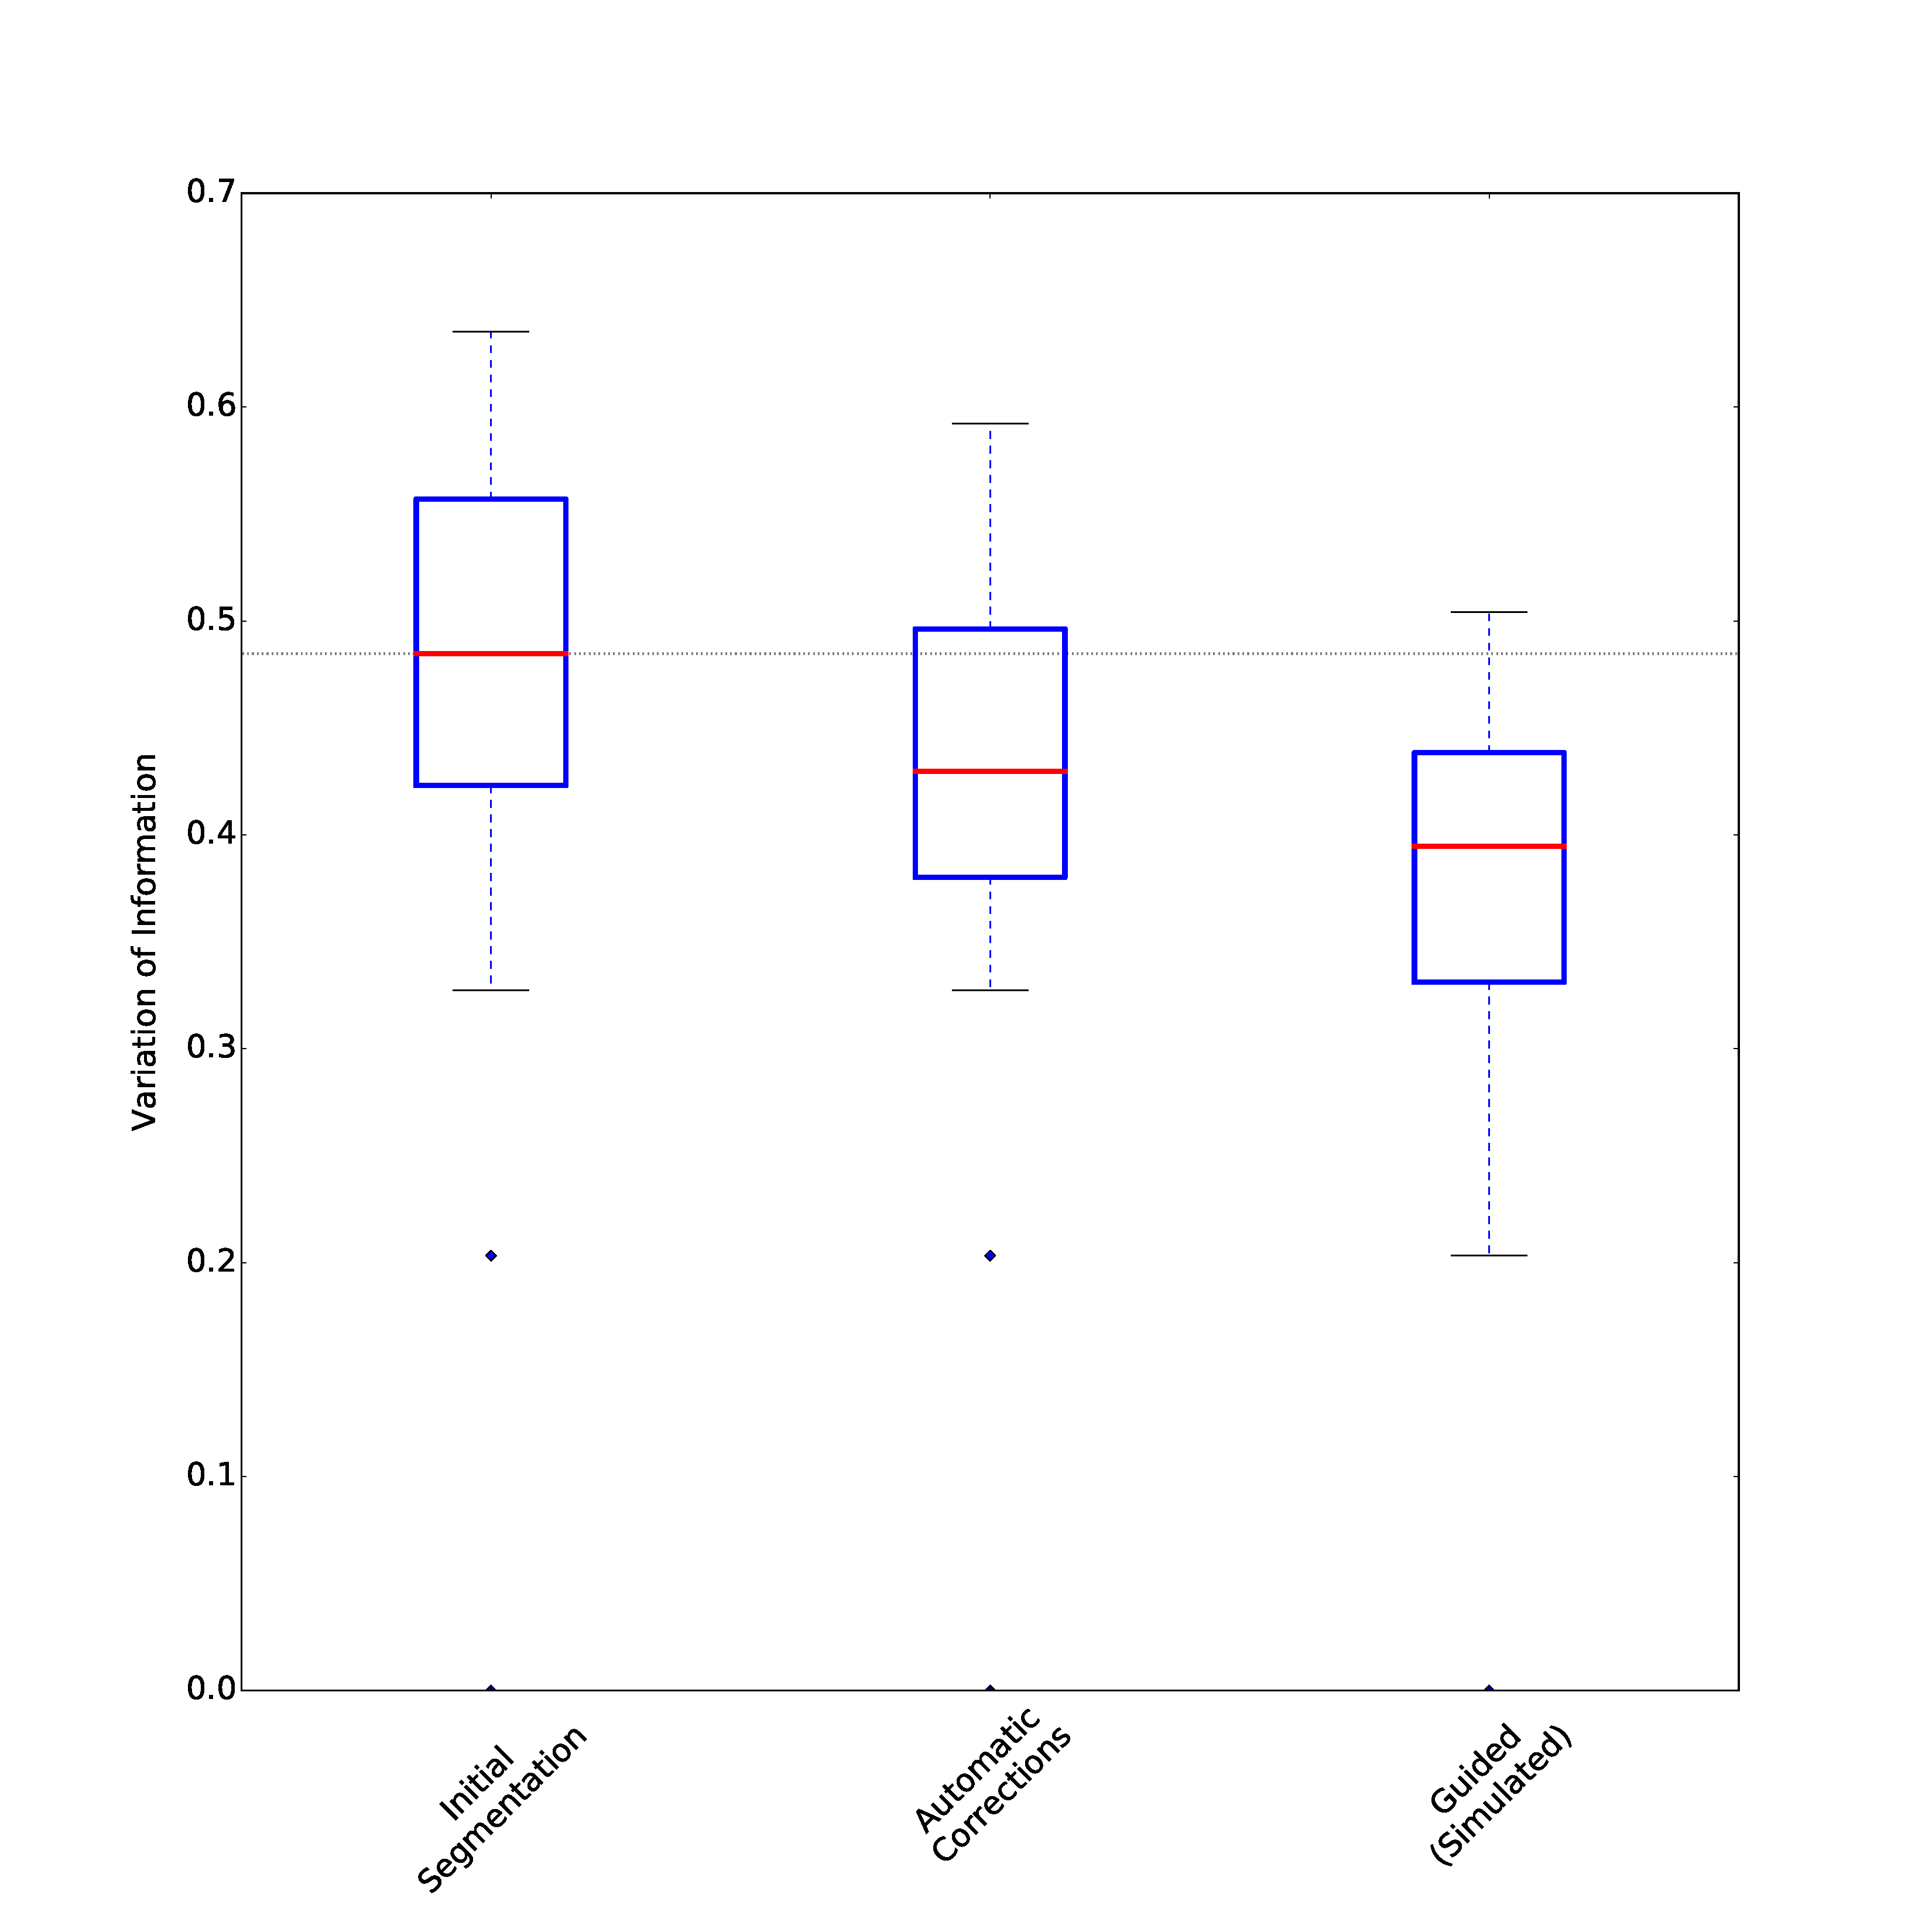
\includegraphics[width=0.49\textwidth]{gfx/cylinder_vi.pdf}
    }
    \hfill
    \subfloat[Variation of Information per Correction\label{fig:cylinder_vi}]{%
      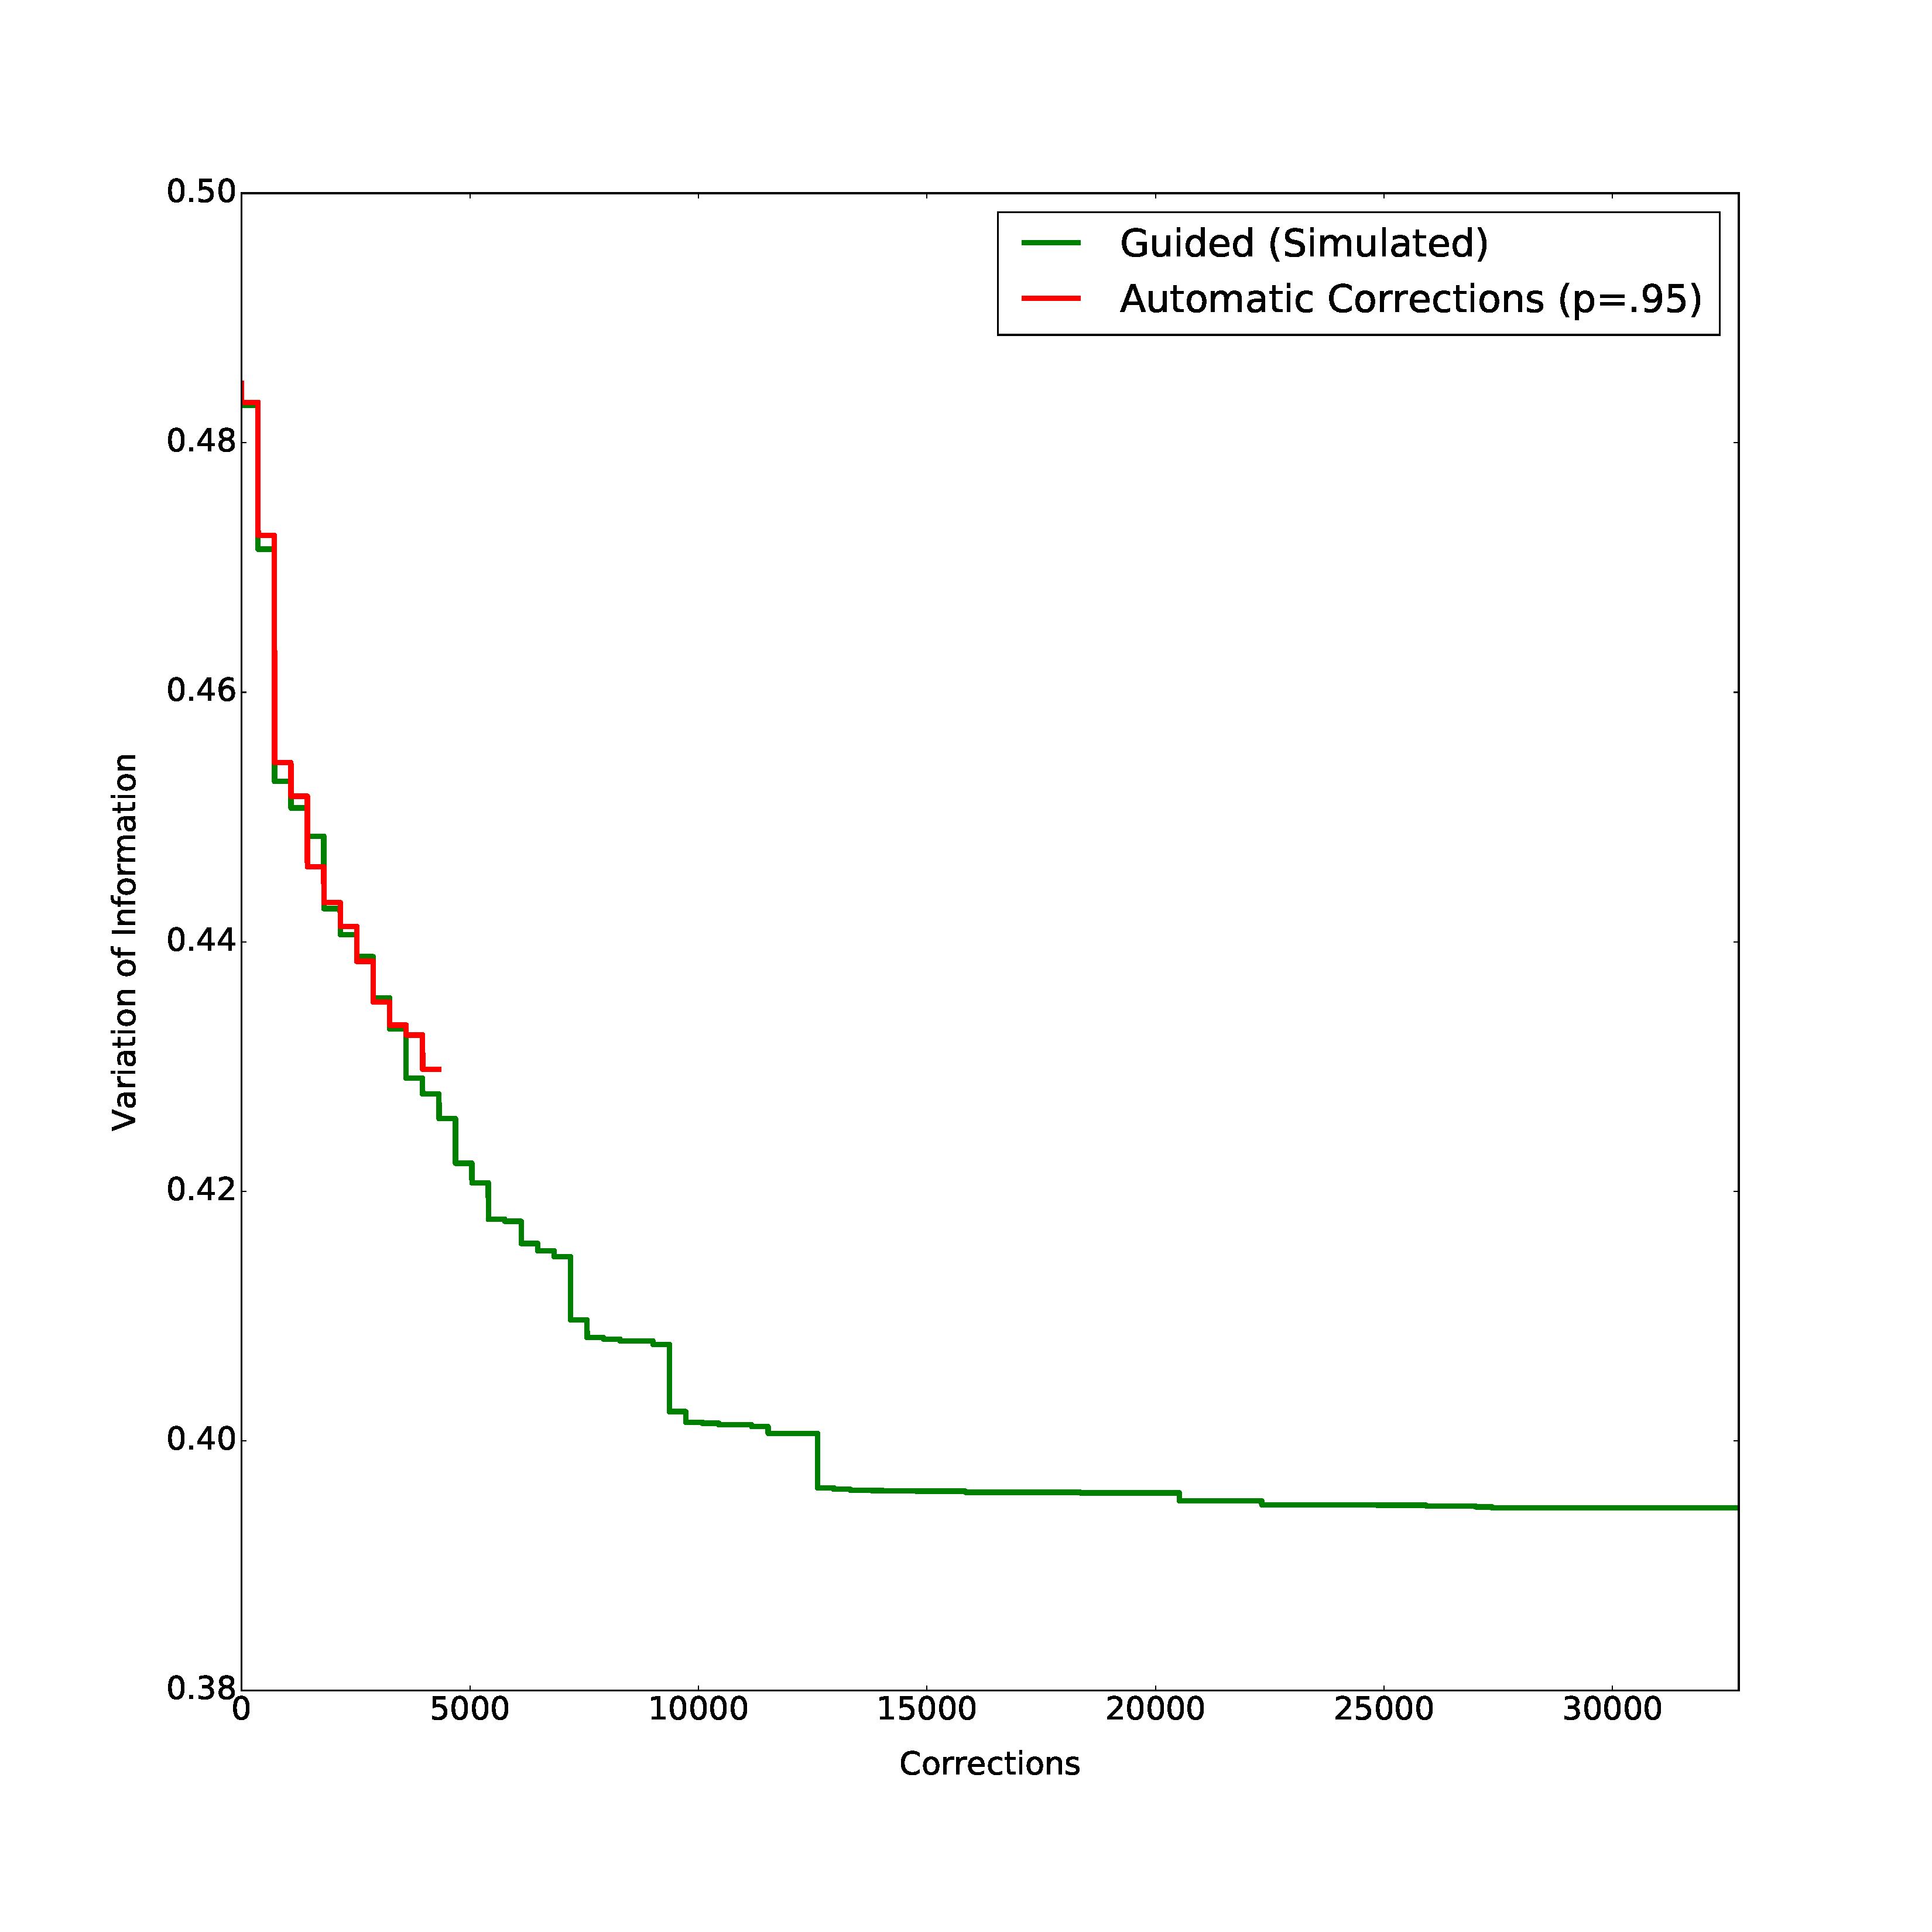
\includegraphics[width=0.49\textwidth]{gfx/cylinder_combined_vi.pdf}
    }
	\caption{Results of our simulated experiment on a larger dataset ($2048\times2048\times50$ voxels). Lower VI scores are better. (a) The initial segmentation is reduced by both fully-automatic correction ($p_t=.95$) and our simulated user. (b) We compare the change in VI measure for each individual correction. The automatic correction stops once the threshold $p_t$ is reached.}
\label{fig:cylinderresults}
\end{figure*}


\begin{figure}[hb]
 \centering
    \subfloat[Split error]{%
      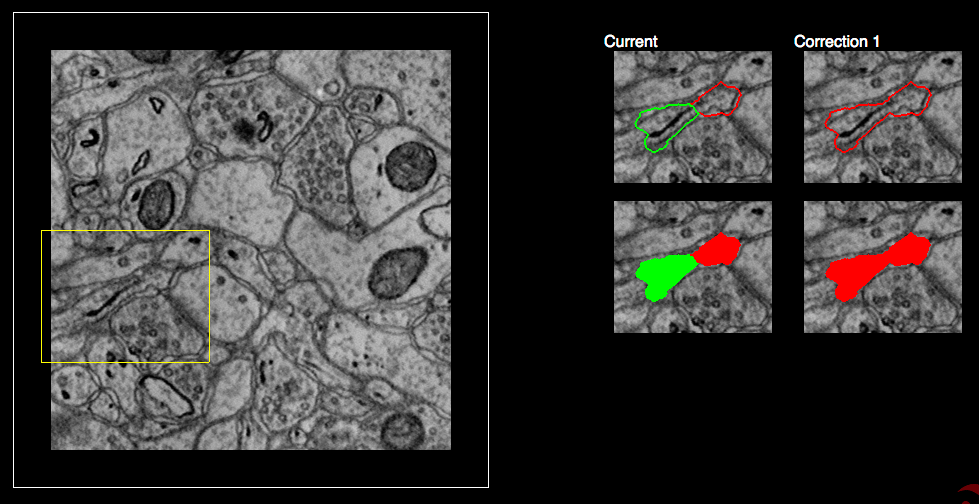
\includegraphics[width=0.95\textwidth]{gfx/proto_split.png}
    }
    \hfill
    \subfloat[Merge error]{%
      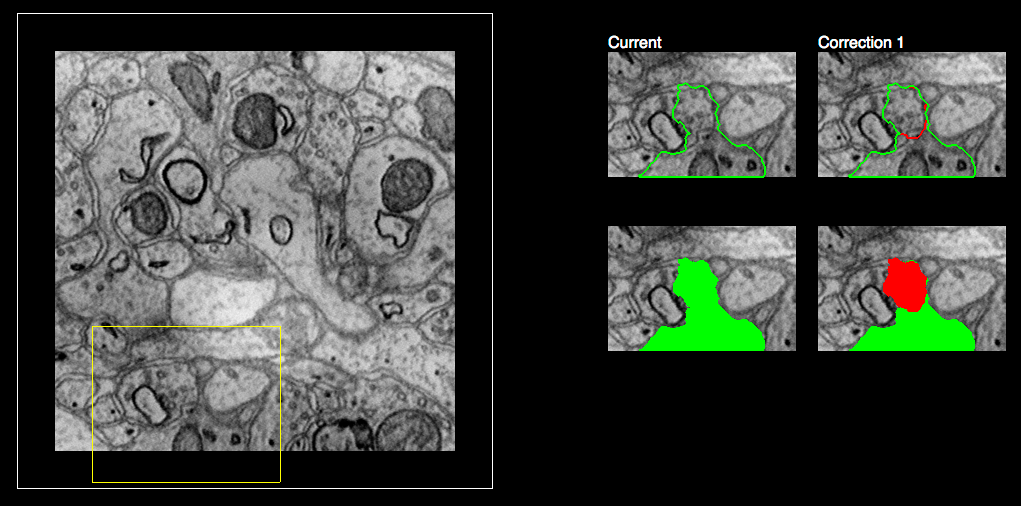
\includegraphics[width=0.95\textwidth]{gfx/proto_merge.png}
    }
	\caption{Our web-based user interface includes a slice overview with the relevant area highlighted in yellow. The interface shows (a) a split error with a suggested correction as well as (b) a merge error with correction. The user selects whether to accept a correction or to discard it.}
\label{fig:prototype}
\end{figure}

\section{Evaluation}
\label{sec:evaluation}




We evaluate our split and merge error detection and correction recommendation in the context of interactive proofreading tools: to direct users to regions with a high probability of error and to suggest corrections (Fig.~\ref{fig:results}). For comparison, we take publicly available mouse cortex data of the same kind as our training data. We perform two experiments: first, we compare our approach with previously reported proofreading results using real-world measurements and second, we evaluate guided proofreading in a simulated context with a much larger dataset.

\subsection{Comparison Study}
\label{sec:comparisonstudy}
For our first experiment, our dataset is part of the ISBI 2013 challenge training dataset ($1024\times1024\times100$ voxels) which was acquired using a serial section scanning electron microscope (ssSEM) with a resolution of $6\times6\times30\, nm$ per voxel. We use the available manually-labeled ground truth to score our approach using the variation of information (VI) metric, which is closely related to mutual information. VI is a measure of the distance between two clusterings, where lower VI numbers are better. Since our classifiers are trained on 2D image slices, we perform all evaluations on slices rather than 3D volumes.



\paragraph{Guided proofreading.}
Recently, Haehn et al.~discussed requirements for interactive proofreading and evaluated three different tools on connectomics data in a study with naive users~\cite{haehn_dojo_2014}. This study asked users to spend 30 minutes proofreading split and merge errors with the different tools to improve upon the automatic segmentation. The best performing tool in their evaluation was Dojo. We use their findings and their user-generated proofreading result data, which they kindly provided, as a baseline for the evaluation of our method.
%The authors performed a non-expert user study and stated that their software Dojo provides better results than other tools due to a minimalistic user interface and sophisticated 3D volume rendering.
Haehn et al. perform their user study on the most representative sub-volume ($400\times400\times10$ voxels) in terms of distribution of object size. For optimal comparison, we use exactly the same data and time constraints. We asked two experts to perform the proofreading task using our system (Fig.~\ref{fig:prototype}).

In addition, we simulate a user for proofreading correction. We assume that all classification has been computed ahead of time, and that the user is presented with a stream of error corrections to assess. The assessment is simulated by comparing the VI before and after each performed correction. Corrections are accepted only when VI reduces, and we test this across different user error rates (Fig.~\ref{fig:results}). In Haehn et al., the proofreading time was limited to 30 minutes, and human participants performed 59 corrections on average ($\approx30$ seconds per correction). In our scenario, users do not need to visually find errors and manually correct them, and from real-world user performance we observed an average decision time of $3.2$ seconds. For our simulated user, we assume each correction assessment takes 5 seconds (360 assessments in 30 minutes). Split errors are likely to take less time than this; however, merge errors are harder to assess, as the user must select between the top 5 candidate boundaries. Since the performance between human participants of Haehn et al.'s user study shows large variation within the average performance among all users (VI improvement: $-0.0582$), we present the best performing Dojo user (VI improvement: $0.0102$) as our baseline. The average VI improvement of two experts using our system is $0.0528$. For our simulated user, the VI improvement is $0.0768$ (Fig.~\ref{fig:results}). In total, our classifier predicted 18 merge and 842 split errors in the data.


%, and we test this across different user error rates







\paragraph{Random recommendations.} We decided to test a classifier with random performance in comparison to our learned CNN. For split errors, the simulated user is presented with randomly picked boundaries, which they can accept or reject. For merge errors, the simulated user is presented with 5 randomly selected boundaries from the interior of the segmented region. Around 80\% of all presented regions did not need to be corrected. Hence, the median VI did not decrease much (VI improvement: $0.0011$). The significantly worse performance of this approach demonstrates that our network is informative to the user.

\paragraph{Automatic correction.} As a comparison, we also perform automatic correction. During training, we define a probability threshold $p_t=0.95$ for automatic split correction based on CNN probability from the test set. Then, for automatic correction, we apply both classifiers to produce lists of split and merge errors sorted by confidence. First, we correct merge errors with $\max(1-p)$, followed by split error correction using $p_t$. The total time for correcting all errors was 17 minutes on a 3.2 GHz Quad-core Intel Xeon with an NVIDIA GeForce Titan (merge error correction 15min, split error correction 2min). The median VI improvement in comparison to the ground truth was $0.02$ (Fig.~\ref{fig:results}). This is not surprising, as the problem is very challenging, and this motivates the need for human-in-the-loop proofreading tools.

\subsection{Simulated Experiment}

For our second experiment, we proofread 50 slices of the blue 3-cylinder cortex volume of Kasthuri et al. \cite{kasthuri2015saturated}. The data was not seen by the network before and includes 2048 x 2048 x 50 voxels with a total number of 33,076 labeled objects. Since interactive proofreading of such a large dataset would consume a significant amount of time, we restrict our experiment to a simulated user and to automatic corrections. Similar to our comparison study (see section \ref{sec:comparisonstudy}), the simulated user assesses a stream of errors by comparing VI before and after each performed correction. As before, corrections are only accepted when VI reduces. In contrast to our time limit in the comparison study, the simulated user proofreads until all objects in the volume were assessed. For automatic corrections, we use our defined probability threshold $p_t=0.95$. 
Based on a time budget of 5 seconds per correction, the proofreading process for a real user would in theory take over 45 hours for this dataset. The total time for automatically correcting all errors was $\approx6$ hours on a 3.2 GHz Quad-core Intel Xeon with an NVIDIA Geforce Titan. The total time for the simulated user including the VI calculations after each assessment was $\approx10$ hours. Both approaches significantly reduce the VI in comparison to the initial segmentation by 0.0901 for the simulated user and by 0.0549 automatically. Results are shown in Fig. \ref{fig:cylinderresults}. 